% !TEX encoding = UTF-8
% !TEX TS-program = pdflatex
% !TEX root = ../tesi.tex

%**************************************************************
\chapter{Processi e metodologie}
\label{cap:processi-metodologie}
%**************************************************************
\intro{Introduzione al capitolo}\\
In questo capitolo andranno affrontati i processi e le motodologie affrontate per lo sviluppo del progetto. Più precisamente verranno descritti i principi cardine dell’\textit{Agile programming}
e successivamente verrà illustrato come questi siano stati applicati durante l'attività di stage.\\

%**************************************************************
\section{Processo sviluppo prodotto}
Lo stage presso Siav mi ha permesso di entrare concretamente a contatto con una metodologia di gestione di progetto vista durante il corso di Ingegneria del Software: la metodologia Agile.
\subsection{Metodologia Agile}
La metodologia Agile si riferisce ad un insieme di metodi di sviluppo del software emersi nei primi anni 2000 e fondati su un insieme di principi comuni derivati dai principi del "Manifesto per lo sviluppo agile del software". 
Fra le pratiche presenti vi è la formazione di team di sviluppo piccoli, lo sviluppo iterativo e incrementale, la pianificazione adattiva e il rapporto costante e diretto con il proponente durante il processo di sviluppo.
\begin{figure}[!h] 
	\centering 
	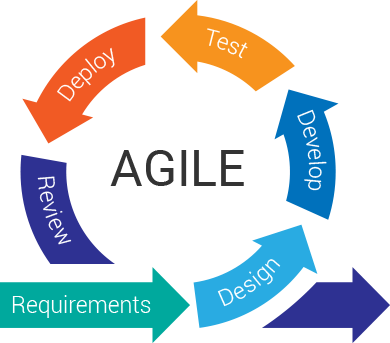
\includegraphics[width=0.3\columnwidth]{agile} 
	\caption{Ciclo dei vita della metodolia agile}
\end{figure}
\subsection{Metodologia Agile in relazione allo stage}
Durante il periodo di stage, tramite il supporto del tutor e del team in cui sono stato inserito ho cercato di apprendere nella miglior maniera possibile i principi cardine dell'\textit{Agile programming}. Non avendo mai avuto l'occasione prima d'ora di approcciarmi a tale metodologia è stato impegnativo entrare nei suoi meccanismi pratici e nelle sue dinamiche. Tuttavia sono riuscito, almeno in parte, a comprendere alcune importanti metodologie che sono state applicate durante tutto il periodo di stage:
\begin{itemize}
	\item Stand-up daily meeting : Ogni giorno, solitamente la mattina, vi era un momento di confronto con tutti i membri del team in merito alle attività da svolgere durante la giornata, tenendo in considerazione eventuali criticità che sarebbero putute emergere ed eventuali problematiche che sono state riscontrate nella giornata prcedente.
	\item Stand-up weekly meeting: Ad inizio settimana veniva discussa con il tutor la pianificazione del lavoro per la settimana, analizzando se il percorso intrapreso fosse congruo con gli obiettivi preposti.
	\item Software over documentation: Durante tutto il periodo di progetto è stata data maggior  priorità al software sviluppato piuttosto che alla documentazione. È stata racchiusa ogni macro attività all'interno di brevi note per poter tener traccia delle scelte fatte e delle attività svolte, prive di formalismi rispetto alla documentazione classica. Tramite ciò è stato possibile dare una maggior attenzione allo sviluppo, concentrandosi maggiormente sulle richieste del proponente, mantenendo però una cronologia delle attività svolte e dalla scelte adottate in modo sintetico ma preciso.
	\item Dialogo continuo con il cliente: Il cliente nel mio caso veniva individuato dal tutor aziendale (team leader del reaprto R\&D). Il dialogo è stato frequente e mirava ad aggiornarlo frequentemente riguardo allo stato di avanzamento dei processi per verificare se le attività che mi ero prefissato erano in linea con le aspettative.
\end{itemize}